% !TEX root = ./informe.tex
\section{Problema 4: Heurística de búsqueda local}

\subsection{Descripción del algoritmo}

Después de aplicar la heurística de búsqueda golosa sobre el problema obtenemos un grafo en el que puede haber conflictos. Esta segunda heurística que desarrollamos se aplica sobre instancias del problema donde ya hay un color válido asignado a todos los nodos. Se trata, entonces, de reducir la cantidad de conflictos de la instancia.

La heurística de búsqueda local define una "vecindad" del problema como una modificación pequeña que se hace sobre el grafo, haciendo un análisis local sobre un nodo o arista. Hemos definido dos vecindades del problema.

El cuerpo principal del algoritmo itera por todos los conflictos del grafo, aplicando una vecindad sobre cada arista que representa a un conflicto.

\subsubsection{Vecindad 1}

Esta vecindad toma una arista en conflicto\footnote{Es decir que ambos nodos de la arista tienen el mismo color.} e intenta modificar el color de uno de los dos nodos, tratando de reducir la cantidad total de conflictos.

\begin{algorithm}[H]
\caption{Vecindad 1.}
\label{vecindad1 pseudocode}
La vecindad opera sobre una arista que recibe como parámetro. Llamaremos a esta arista \texttt{conflicto}. Los dos nodos unidos por esta arista serán N1 y N2:
\begin{enumerate}
 \item crear un diccionario para ambos nodos. El diccionario tendrá como key a los colores del nodo, y como valor una lista de vecinos del nodo que tienen asignado ese color. Llamaremos a estos diccionarios \texttt{conflictosPorColorN1} y \texttt{conflictosPorColorN2}.
 \item tanto para N1 como para N2, iteramos sobre su lista de colores posibles y llenamos los diccionarios conflictosPorColorN1 y conflictosPorColorN2 de manera tal que para cada color posible de ambos nodos, tenemos una lista vacía de vecinos.  // O(c), pues cada nodo tiene a lo sumo $c$ colores posibles.
 \item Luego iteramos la lista de vecinos de N1. Si el color del vecino es uno de los colores posibles de N1, agregaremos este vecino a la lista de conflictosPorColorN1[color_del_vecino]. // O($n$), pues cada nodo tiene a lo sumo $n-1$ vecinos.
 \item Hacemos lo mismo para los vecinos de N2. // O(n)
 \item Ahora buscamos dentro de conflictosPorColorN1 al color que genera menos conflictos (su lista es la más corta). // O(c)
 \item Hacemos lo mismo para conflictosPorColorN2. // O(c)
 \item De esos dos elegimos al menor. Si la cantidad de conflictos es menor a la que se tiene dejando todo como está, cambiamos el color del nodo. Si no, la vecindad no sirvió y no hacemos modificaciones en el grafo. // O(n), ya que para modificar el color de un nodo debemos actualizar una estructura de datos que tiene 
\end{enumerate}
\end{algorithm}


La complejidad calculada para la vecindad 1 es de $\mathcal{O}(n + c)$.


\subsubsection{Vecindad 2}

Esta vecindad toma una arista en conflicto e intenta intercambiar el color de uno de los nodos del confclito con el color de algún vecino suyo.

\begin{algorithm}[H]
\caption{Vecindad 2.}
\label{vecindad2 pseudocode}
La vecindad opera sobre una arista que recibe como parámetro. Llamaremos a esta arista \texttt{conflicto}. Los dos nodos unidos por esta arista serán N1 y N2:
\begin{enumerate}
 \item Para cada N de \{ N1, N2 \} hacemos:
 \begin{enumerate}
   \item obtengo una lista de vecinos de N con los cuales puedo intercambiar color. Son aquellos vecinos que cumplen las siguientes tres condiciones:	// O(n) iteraciones
   \begin{enumerate}
    \item Su color es distinto del color de N.			// O(1)
    \item Su color está dentro de la lista de colores posibles de N	// O(c)
    \item Tienen al color de N dentro de su lista de colores posibles.	// O(c)
   \end{enumerate}
   \item Para cada vecino de N con el que puedo intercambiar color, calculo la cantidad de conflictos que solucionaría al hacer ese intercambio de colores. // O($n^2$)
   \item Elijo al vecino que me solucionaría la mayor cantidad de conflictos. // O(n)
 \end{enumerate}
 \item De entre los dos intercambios posibles (N1 por su vecino, o N2 por su vecino), elijo el que solucione la mayor cantidad posible de conflictos. // O(1)
 \item Realizo el cambio, actualizando la lista de conflictos del grafo.\footnote{Es posible que no encuentre vecinos que solucionen conflictos, o que hacer el intercambio de colores me genere más conflictos que los que previamente tenía. En ese caso, no se realiza el cambio.} // O(n)
 
\end{enumerate}
\end{algorithm}

La complejidad calculada para la vecindad 2 es de $\mathcal{O}(n \cdot c + n^2)$.

\subsubsection{Cantidad total de iteraciones}

Como dijimos, el cuerpo principal del algoritmo itera sobre todos los conflictos hallados al inicio. Con lo cual, la complejidad total del algoritmo debe ser de $\mathcal{O}(conflictos \cdot (n+c)$ para la vecindad 1, y $\mathcal{O}(conflictos \cdot (n \cdot c + n^2))$ para la vecindad2. Y siempre la cantidad de conflictos es $\mathcal{O}(m)$.

\subsection{Experimentación}

\subsubsection{Tiempos de ejecución}

Para verificar experimentalmente las cotas de complejidad calculadas, escribimos generadores de grafos al azar y ejecuciones donde vamos generando grafos y resolviéndolos, tomando mediciones. Se puede hallar el código utilizado en el archivo \texttt{ExperimentosComplejidad.java}.

En primer lugar hicimos un análisis en función de la cantidad de nodos con grafos completos. Esto se puede observar en la figura \ref{nodosEj4}. Allí se ve que los tiempos medidos incrementan dentro de la cota definida por la curva de $n^3$. Esto es razonable ya que en un grafo completo la cantidad de aristas es del órden de $n^2$, y la cantidad máxima de colores se dejó fija para estas mediciones.

\begin{figure}[]
	\centering
 	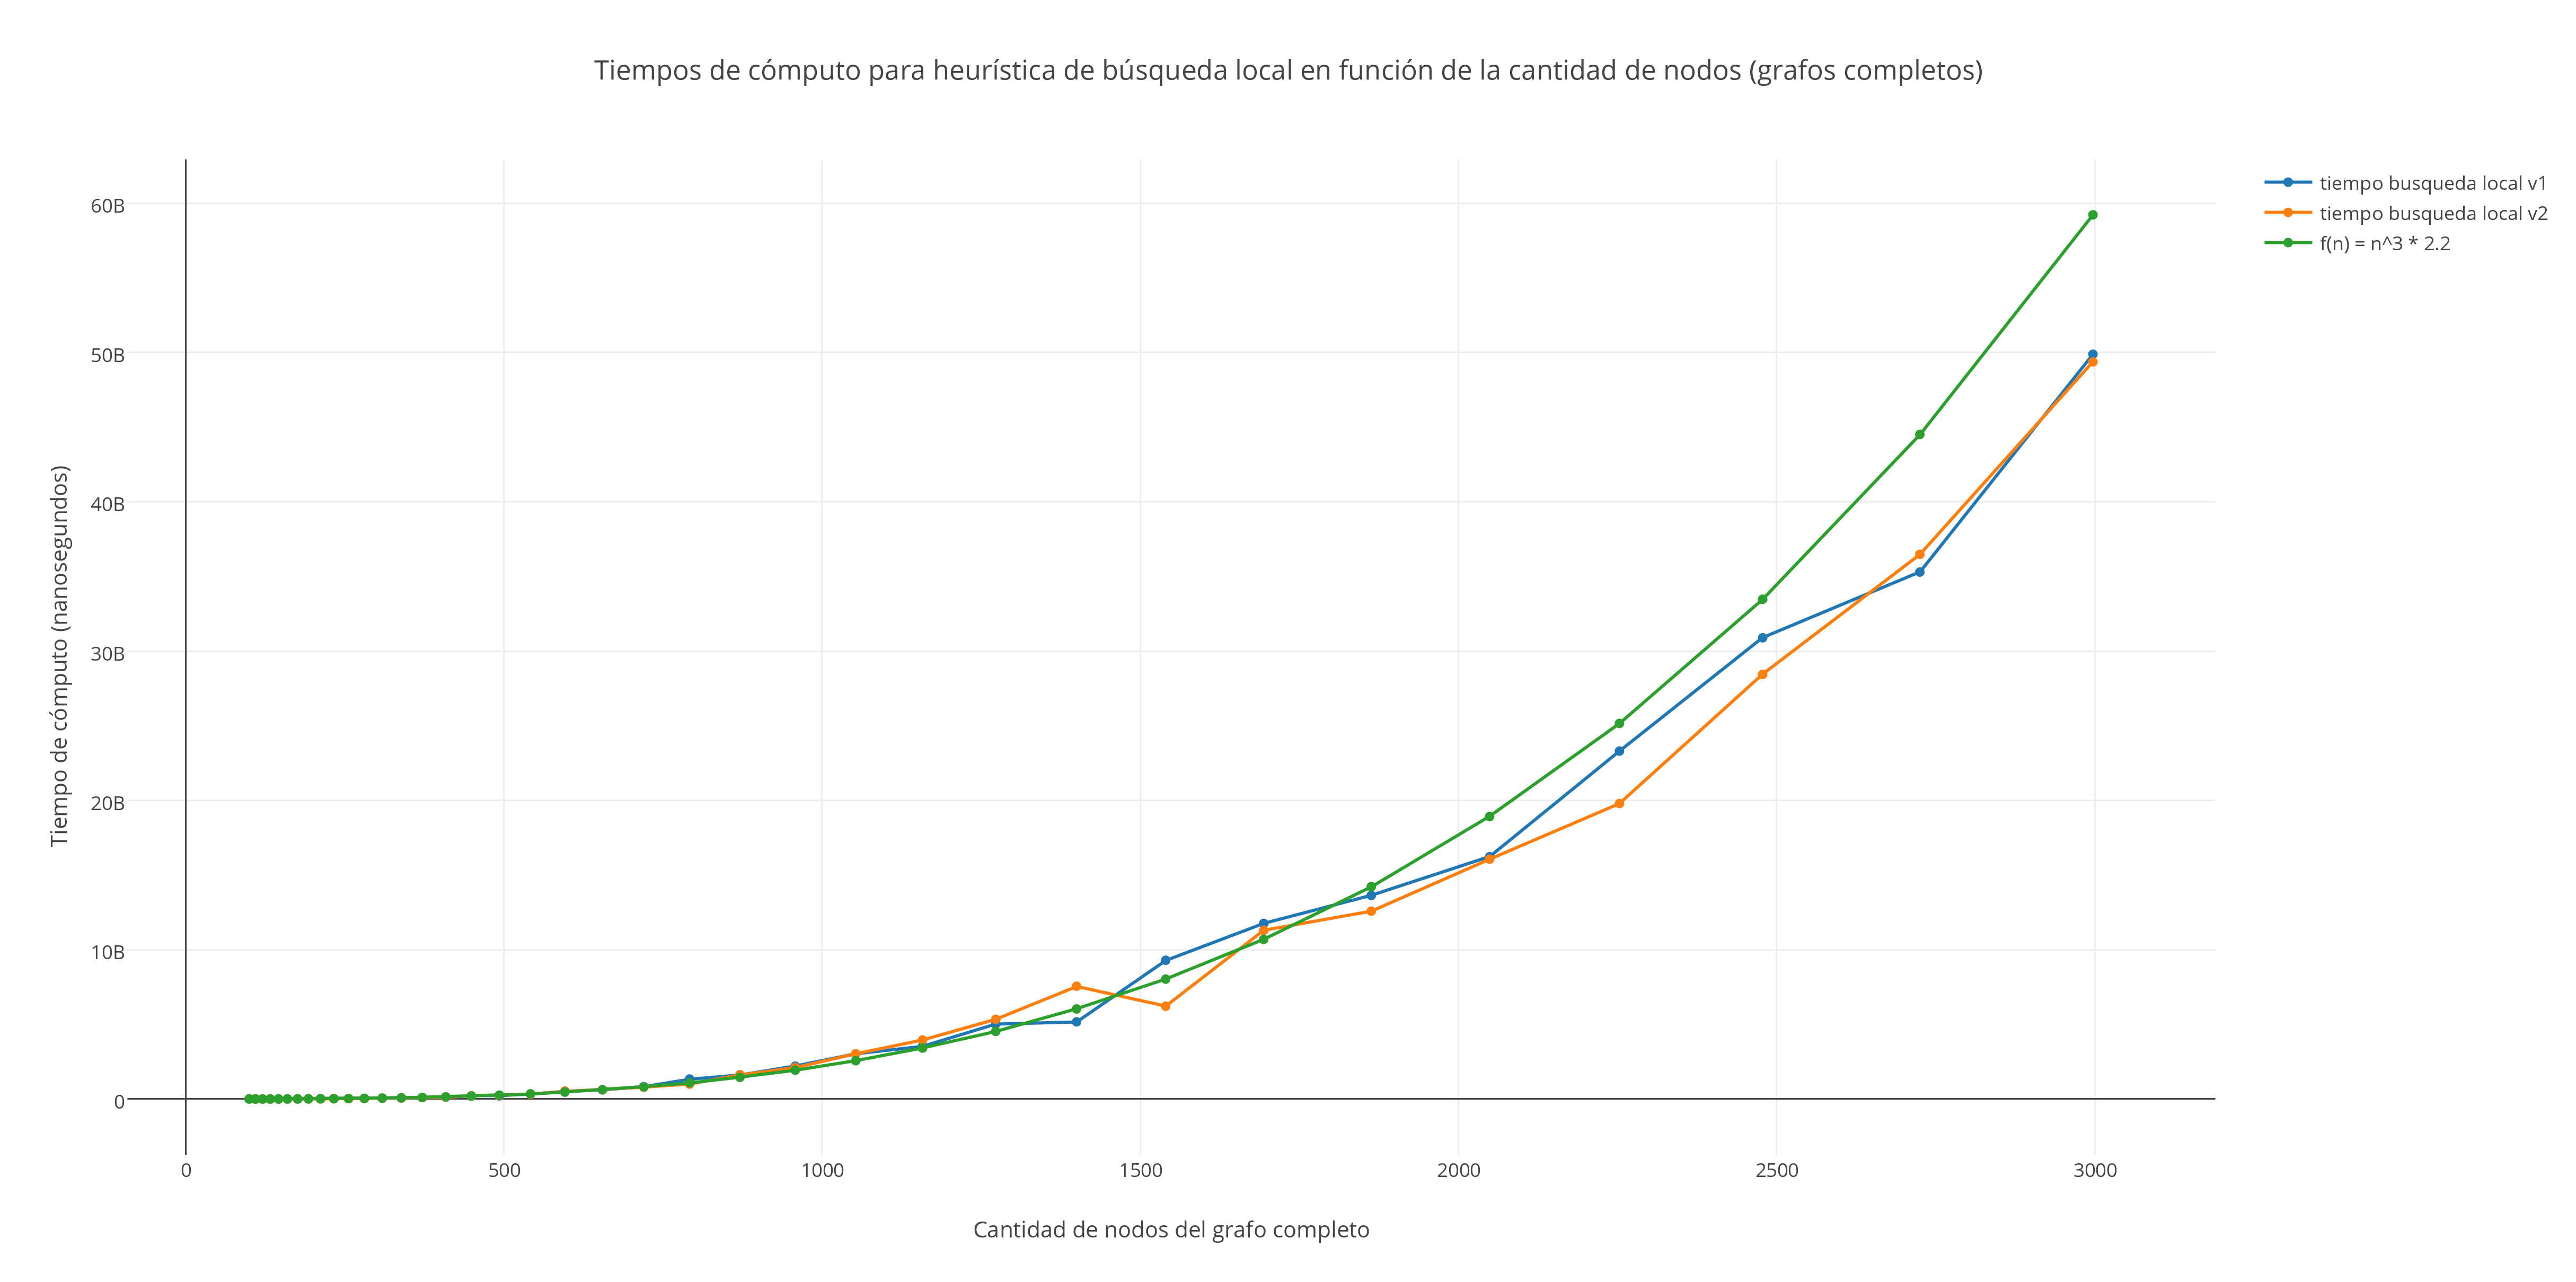
\includegraphics[width=18cm]{imagenes/Ej4/TvsNodos.png}
	\caption{Tiempos de cómputo en búsqueda local en función de la cantidad de nodos.}
	\label{nodosEj4}
 \end{figure}
 
También analizamos cómo variaba el tiempo de cómputo en función de la cantidad total de aristas (figuras \ref{aristasEj4-1} y \ref{aristasEj4-2}). Estas gráficas revelan que la complejidad medida no coincide con la complejidad que calculamos a partir del análisis del código. La figura \ref{aristasEj4-2}, en particular, estaría indicando que el tiempo de ejecución del algoritmo, con cualquiera de las dos vecindades es $\mathcal{O}(m \cdot conflictos)$, cuando de nuestro análisis surgía que la complejidad de la vecindad 1 era de $\mathcal{O}(conflictos \cdot (n+c)$  y de $\mathcal{O}(conflictos \cdot (n \cdot c + n^2))$ para la vecindad 2.

\begin{figure}[]
	\centering
 	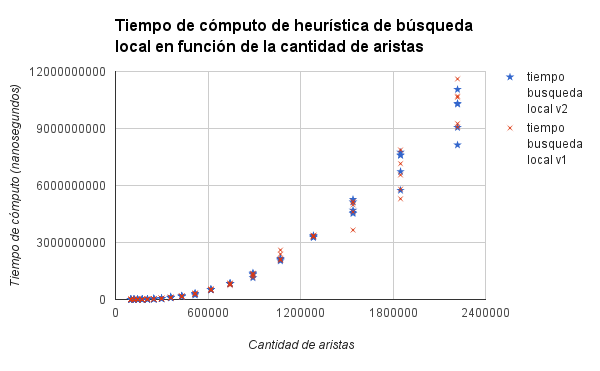
\includegraphics[width=18cm]{imagenes/Ej4/TvsAristas1.png}
	\caption{Tiempos de cómputo en búsqueda local en función de la cantidad de aristas.}
	\label{aristasEj4-1}
 \end{figure}
 
 \begin{figure}[]
	\centering
 	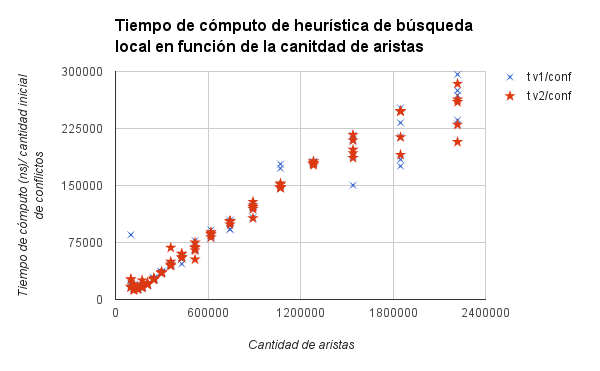
\includegraphics[width=18cm]{imagenes/Ej4/TvsAristas2.png}
	\caption{Tiempos de cómputo por conflicto (promedio) en búsqueda local en función de la cantidad de aristas.}
	\label{aristasEj4-2}
 \end{figure}
 
  \begin{figure}[]
	\centering
 	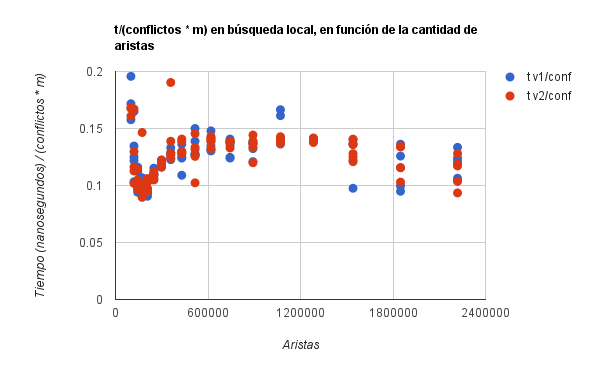
\includegraphics[width=18cm]{imagenes/Ej4/TvsAristas3.png}
	\caption{T/(conflictos * m) en función de la cantidad de aristas.}
	\label{aristasEj4-3}
 \end{figure}
 
 Y en función de la cantidad total de colores.
 
  \begin{figure}[]
	\centering
 	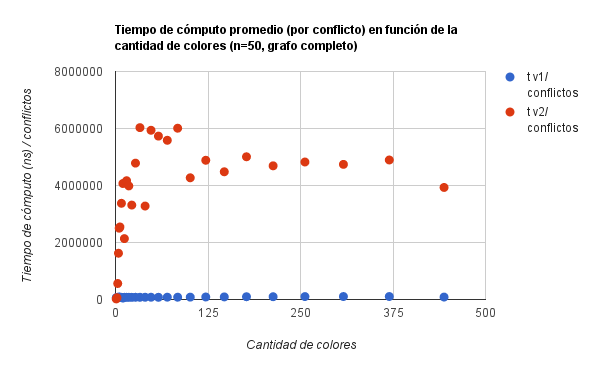
\includegraphics[width=18cm]{imagenes/Ej4/TvsColores.png}
	\caption{Tiempos de cómputo en búsqueda local en función de la cantidad de colores.}
	\label{coloresEj4-2}
 \end{figure}
 
 También hicimos una comparación entre la cantidad de conflictos que se resuelven con las distintas heurísticas.
 
  \begin{figure}[]
	\centering
 	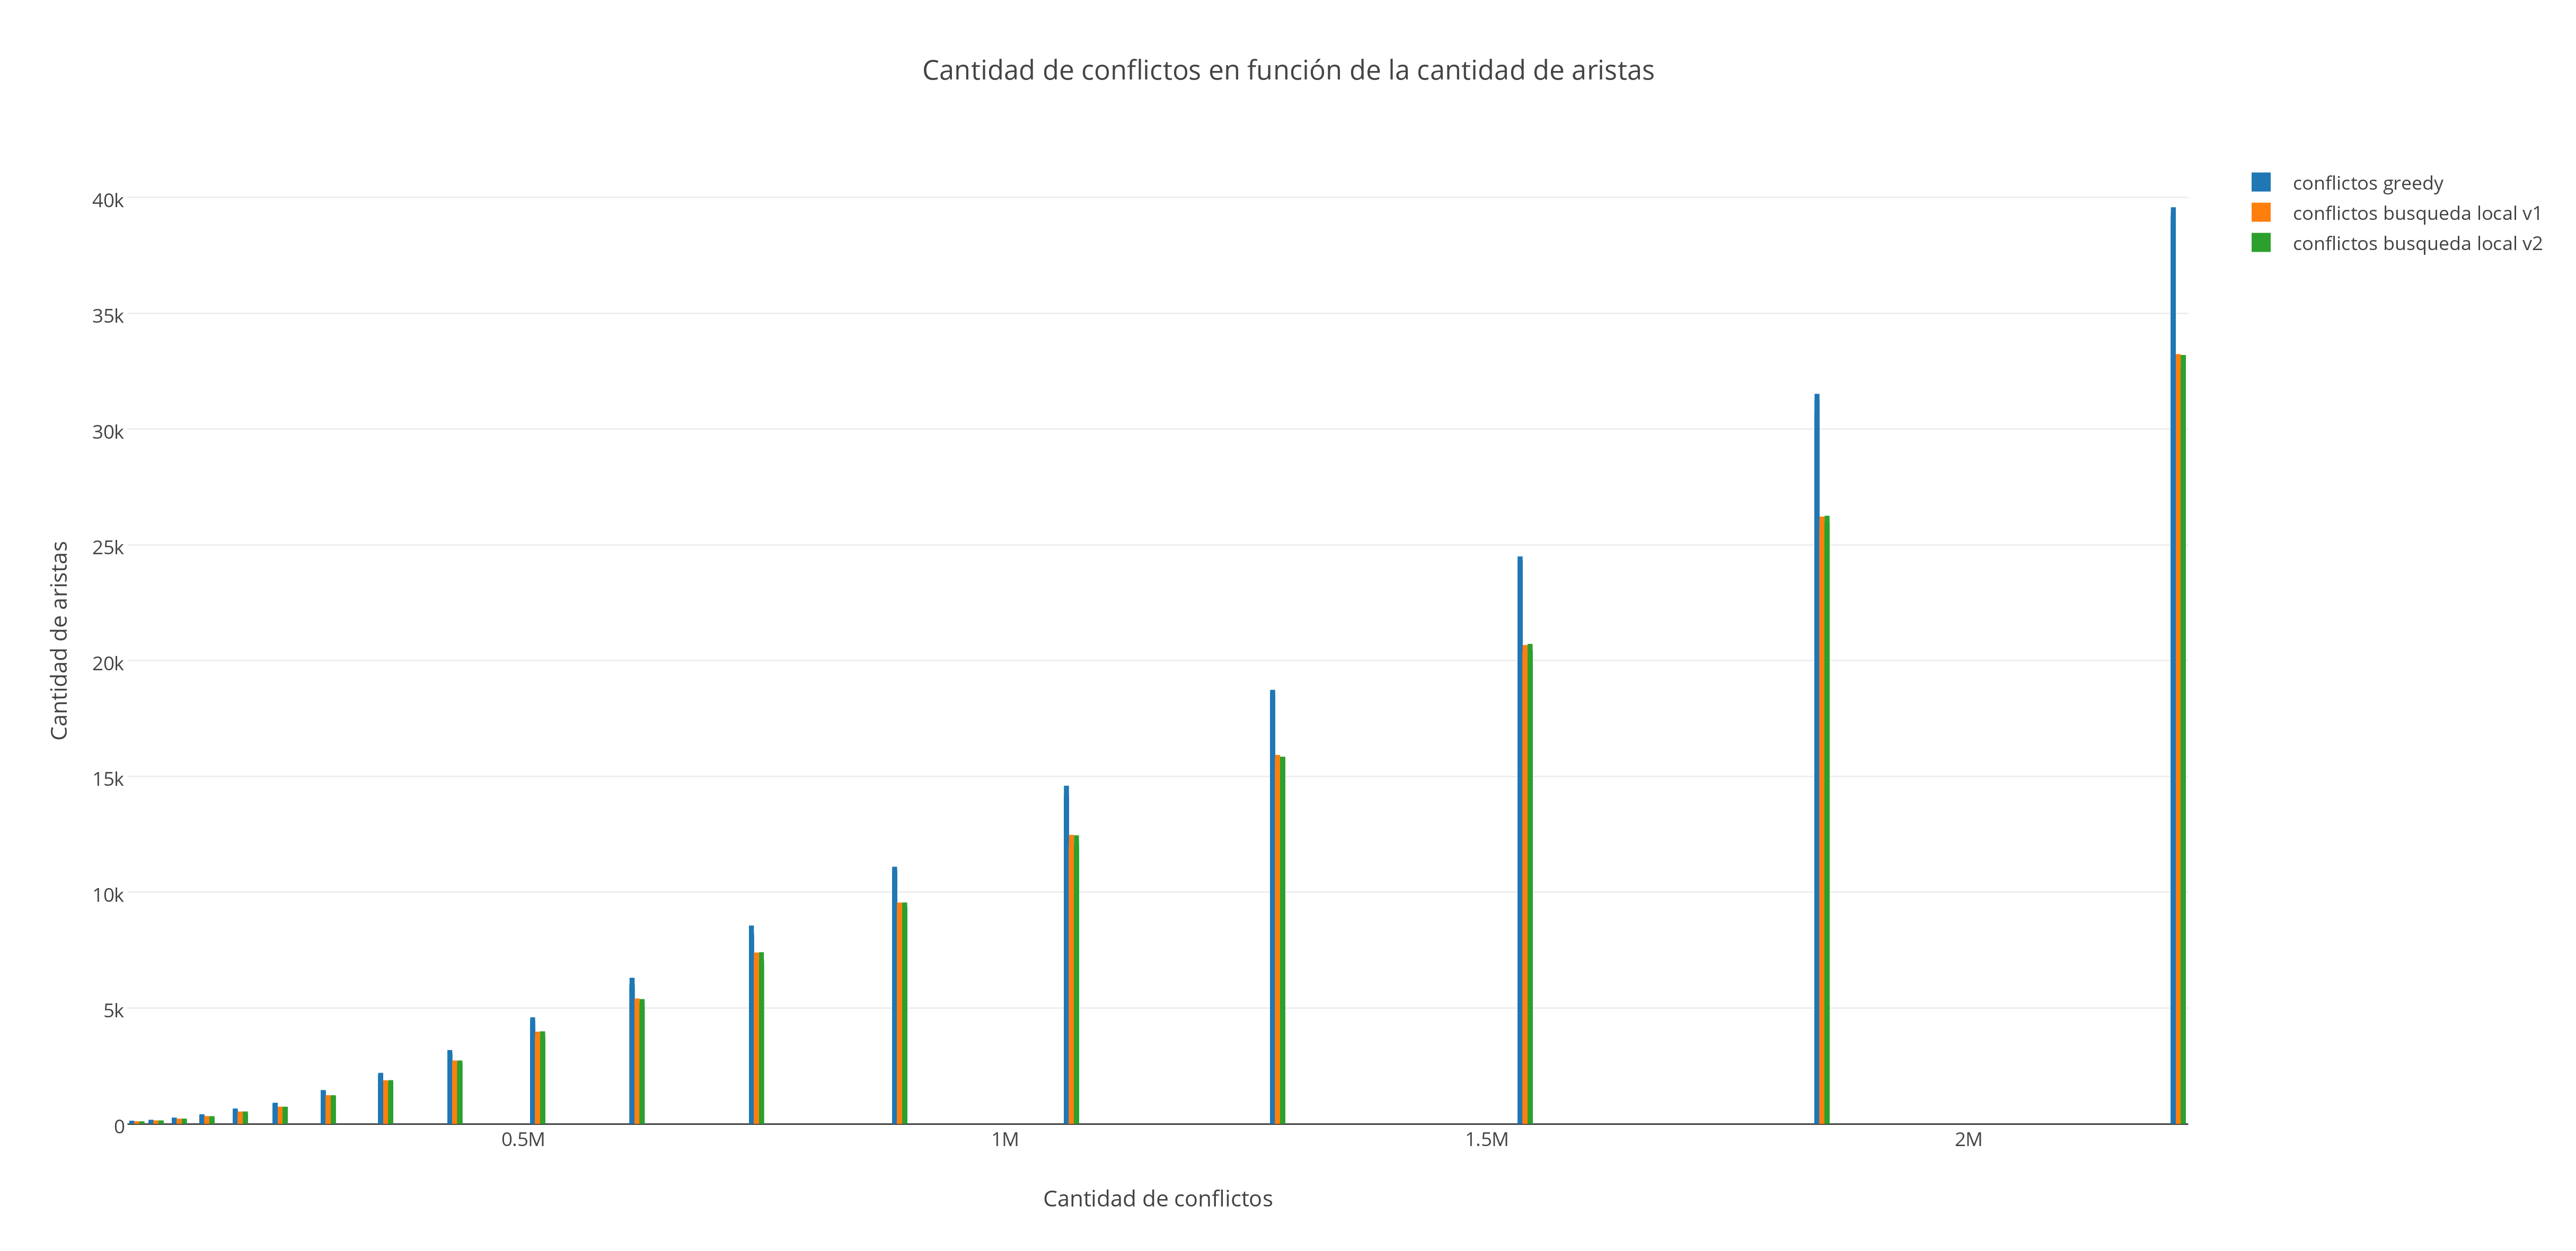
\includegraphics[width=18cm]{imagenes/Ej4/conflictosVsAristas.png}
	\caption{Cantidad de conflictos en el grafo luego de resolver usando distintas heurísticas/vecindades.}
	\label{conflictosEj4}
 \end{figure}
 
\begin{figure}[]
	\centering
 	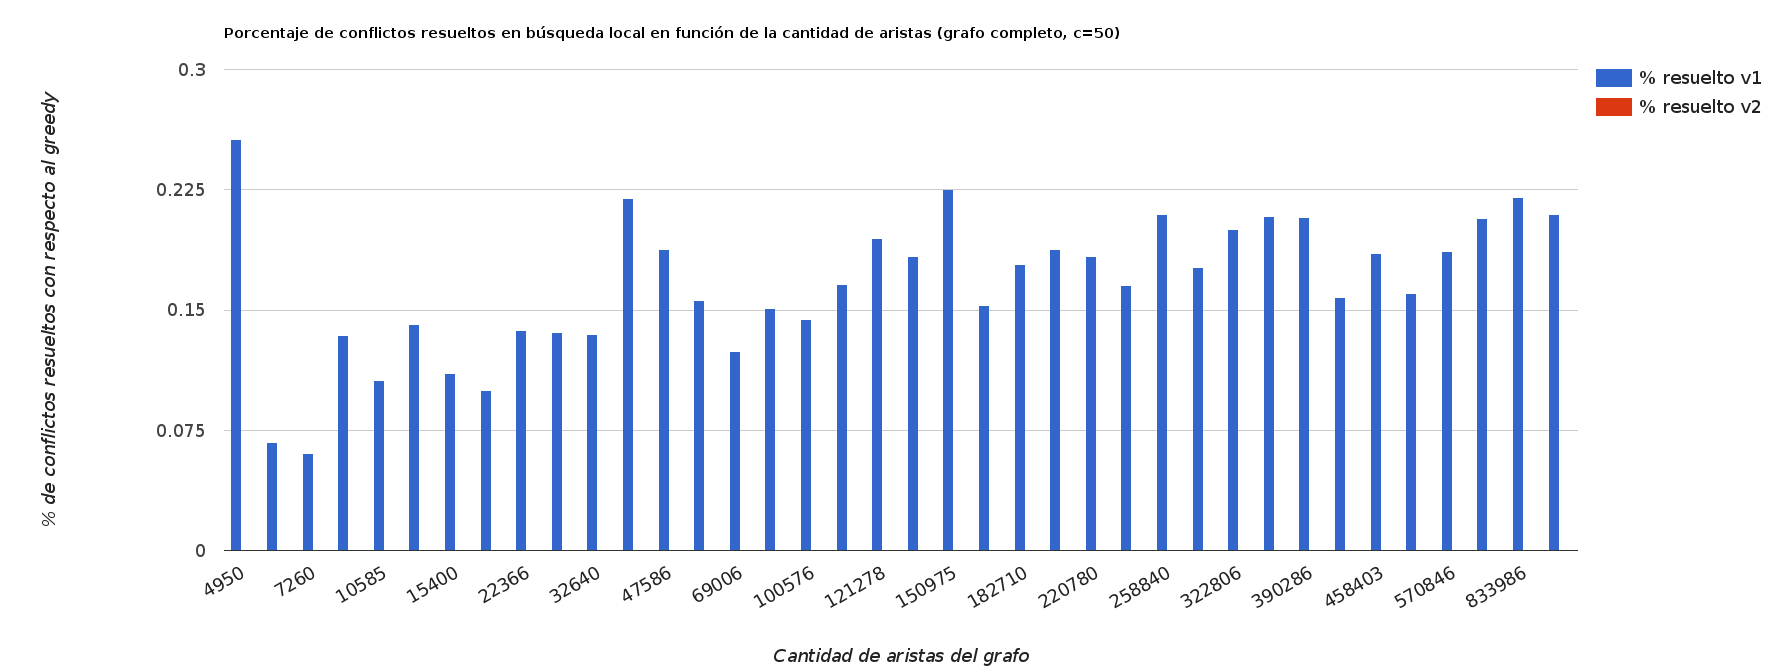
\includegraphics[width=18cm]{imagenes/Ej4/porcentajeConflictosVsAristas.png}
	\caption{Porcentaje de conflictos resueltos por cada vecindad en función de la cantidad de aristas.}
	\label{conflictosEj4-porcentaje}
 \end{figure}

 
 No hubo diferencias apreciables entre la vecindad 1 y la vecindad 2.